% QoS-Aware Emergency Traffic Prioritization - Mini Project Report
% Format: report-format.docx (A4, Times 12 pt, 1.5 spacing, 1-inch margins, justified body)
% Build: pdflatex main.tex  (run twice for the table of contents / lists)
\documentclass[12pt,a4paper]{article}

\usepackage[T1]{fontenc}
\usepackage{mathptmx}                 % Times-like text and math
\usepackage[margin=1in]{geometry}
\usepackage{setspace}
\usepackage{graphicx}
\usepackage{booktabs}
\usepackage{longtable}
\usepackage{array}
\usepackage{tabularx}
\usepackage{float}
\usepackage[font=small,labelfont=bf]{caption}
\usepackage{listings}
\usepackage{xcolor}
\usepackage{fancyhdr}
\usepackage{titlesec}
\usepackage{tikz}
\usetikzlibrary{positioning,arrows.meta,calc}
\usepackage[hidelinks]{hyperref}

\onehalfspacing
\setlength{\parindent}{0pt}
\setlength{\parskip}{6pt}
\setlength{\emergencystretch}{2em}
\renewcommand{\arraystretch}{1.15}

\titleformat{\section}{\Large\bfseries}{\thesection}{0.6em}{}
\titleformat{\subsection}{\large\bfseries}{\thesubsection}{0.6em}{}
\titlespacing*{\section}{0pt}{14pt}{6pt}
\titlespacing*{\subsection}{0pt}{10pt}{4pt}

\pagestyle{fancy}
\fancyhf{}
\renewcommand{\headrulewidth}{0pt}
\fancyfoot[R]{\small Computer Networks Laboratory \quad \thepage}

\lstset{basicstyle=\ttfamily\footnotesize,breaklines=true,columns=fullflexible,
        frame=single,xleftmargin=0pt,showstringspaces=false,aboveskip=6pt,belowskip=6pt}

% Student/guide details are not part of the repository: fill these in before submission.
\newcommand{\ph}[1]{\textbf{[#1]}}
\newcommand{\projtitle}{QoS-Aware Emergency Traffic Prioritization}
\newcommand{\grp}{13}
\newcommand{\panel}{K}
\newcommand{\batch}{K2 and K3}
\newcommand{\code}[1]{\texttt{#1}}
\newcommand{\shot}[3]{% file, caption, label
  \begin{figure}[H]\centering
  \includegraphics[width=0.88\textwidth,height=0.5\textheight,keepaspectratio]{screenshots/#1}
  \caption{#2}\label{#3}\end{figure}}

\begin{document}

%====================================================================
% COVER PAGE
%====================================================================
\pagenumbering{gobble}
\begin{center}

\includegraphics[width=0.45\textwidth]{logo.png}\\[10pt]
{\Large\bfseries Department of Computer Engineering and Technology}\\[18pt]
{\LARGE\bfseries MINI PROJECT REPORT}\\[8pt]
{\large Computer Networks Laboratory (CSE20110)}\\
{\large Laboratory Continuous Assessment 3}\\[26pt]
{\Huge\bfseries \projtitle}\\[26pt]
{\large Submitted by}\\[8pt]
\begin{tabular}{|c|l|l|}\hline
\textbf{Sr. No.} & \textbf{Student Name} & \textbf{PRN}\\\hline
1 & Kaustubh Dube & 1262254051\\\hline
2 & Abhiram Tawalare & 1262241934\\\hline
3 & Shalaka Bhor & 1262242503\\\hline
4 & Charitra Jain & 1262243266\\\hline
\end{tabular}\\[14pt]
Group No. \grp \quad Panel \panel \quad Batch \batch\\[8pt]
Third Year B.Tech. Computer Engineering and Technology\\[20pt]
{\large Under the guidance of}\\
\textbf{Dr.\ Uma Pujeri}\\\textbf{Prof.\ Swati}\\[14pt]
Academic Year 2026--2027\\
Submission Date 22 October 2026
\end{center}
\newpage

%====================================================================
% CERTIFICATE
%====================================================================
\begin{center}
{\large\bfseries Department of Computer Engineering and Technology}\\[10pt]
{\Large\bfseries CERTIFICATE}
\end{center}

This is to certify that the mini-project entitled ``\projtitle'' has been carried out by the
following students of Third Year B.Tech. Computer Science and Engineering, Panel \panel, Batch
\batch, Group No.\ \grp, under my guidance during the academic year 2026--2027.

\begin{center}
\begin{tabular}{|l|l|}\hline
\textbf{Student Name} & \textbf{PRN}\\\hline
Kaustubh Dube & 1262254051\\\hline
Abhiram Tawalare & 1262241934\\\hline
Shalaka Bhor & 1262242503\\\hline
Charitra Jain & 1262243266\\\hline
\end{tabular}
\end{center}

The report is submitted towards the mini-project component of Laboratory Continuous Assessment~3
for the Computer Networks Laboratory course.

\vspace{3cm}
\noindent Faculty Signature \underline{\hspace{5cm}}\hfill \textbf{Dr.\ Uma Pujeri}\\
\hspace*{\fill}Project Guide and Course Faculty\\[1cm]
Date \underline{\hspace{3cm}} \hfill Place: Pune
\newpage

%====================================================================
% PRELIMINARY PAGES
%====================================================================
\pagenumbering{roman}
\setcounter{page}{1}

\section*{Acknowledgement}
\addcontentsline{toc}{section}{Acknowledgement}
We thank our guides Dr.\ Uma Pujeri and Prof.\ Swati and the Department of Computer Engineering and Technology
for the guidance and the laboratory facilities provided for this mini project. We also acknowledge
the public documentation of the IETF Differentiated Services architecture and the Wireshark project,
which we used as technical references while designing the protocol and the verification tooling.

\vfill\hfill Group No.\ \grp
\newpage

\section*{Abstract}
\addcontentsline{toc}{section}{Abstract}
During disasters, alarm and dispatch traffic shares network links with bulk data, and a plain FIFO
queue lets congestion delay or drop the packets that matter most. This project builds a
QoS-aware emergency traffic prioritization system that classifies traffic into emergency, voice,
video and best-effort classes and schedules packets at a congested bottleneck. It contains a custom
UDP-based protocol (QEP) with a 24-byte header, a staged classifier (header, DSCP, UDP port, flow
cache), five schedulers (FIFO, strict priority, WFQ, DRR and a proposed hybrid Emergency Priority
Scheduler, EPS), a discrete-event simulator with nine test cases, a live demonstration with real UDP
sockets and a rate-limited software router, a web dashboard and packet-level verification tools.
Everything is implemented in the Python 3 standard library. In the simulated 10 Mbit/s scenarios,
FIFO fails the emergency, voice and video SLAs under ${\sim}170\,\%$ load (emergency p99 delay
105.5~ms, 2.91\,\% loss), whereas all QoS schedulers keep emergency p99 delay below 10~ms with no loss.
Under a spoofed ``emergency'' flood, strict priority, WFQ and DRR fail the emergency SLA while EPS
passes all three SLAs. The Mininet emulation was written but not executed, and EPS does not solve
voice over-subscription without call admission control.

\textbf{Keywords:} Quality of Service, Emergency Traffic, Packet Scheduling, DiffServ, Weighted Fair Queueing, UDP.
\newpage

\tableofcontents
\newpage
\listoffigures
\newpage
\listoftables
\newpage

%====================================================================
% MAIN MATTER
%====================================================================
\pagenumbering{arabic}
\setcounter{page}{1}

\section{Introduction and Project Objectives}

\subsection{Introduction and Background}
Quality of Service (QoS) mechanisms let a network treat packets differently when a link is
congested. The IETF Differentiated Services (DiffServ) architecture \cite{rfc2474,rfc2475} marks
each IP packet with a 6-bit Differentiated Services Code Point (DSCP) in the IP header, and routers
apply per-hop behaviours (PHBs) selected by that marking, for example Expedited Forwarding (EF,
DSCP~46) for low-latency voice \cite{rfc3246} and Class Selector 6 (CS6, DSCP~48) for network
control and critical signalling. Packet schedulers decide which queued packet is sent next:
strict priority always serves the highest non-empty queue, while fair-queueing schedulers such as
Weighted Fair Queueing (WFQ) \cite{demers1989} and Deficit Round Robin (DRR) \cite{shreedhar1996}
share the link in proportion to configured weights.

Strict priority gives the lowest delay to the top class but can starve lower classes and blindly
trusts packet markings; weighted schedulers prevent starvation but give the top class only its
weight when the link is saturated. This project examines these trade-offs for emergency traffic and
proposes a hybrid that combines strict priority for the critical classes with weighted sharing for
the rest and with policing against false markings.

\subsection{Problem Statement}
In a disaster, alarms, sensor telemetry and dispatch voice share links with bulk data. When the
bottleneck saturates, a FIFO queue gives every packet the same fate, so emergency packets wait
behind (or are dropped together with) best-effort packets. A scheduler that simply trusts the
priority marking can in turn be abused by a flow that falsely claims to be emergency traffic. A
solution must keep emergency and voice delay, jitter and loss within defined limits during
congestion, survive link failures, resist spoofed markings and avoid starving lower classes.

\subsection{Scope}
The system covers a single congested egress port (one router interface) between a LAN with four
traffic sources (voice, video, emergency, bulk) and a server. Traffic is UDP-based; TCP congestion
control, multi-hop topologies, call admission control and authentication of emergency sources are
outside the scope. The same classifier and schedulers are used in three environments: a
discrete-event simulation (10 Mbit/s link), a live demonstration over loopback UDP sockets with a
software router (1 Mbit/s), and a Mininet/\code{tc} script. Delay is one-way (queueing,
serialization and 5~ms propagation).

\subsection{Objectives}
Table~\ref{tab:objectives} lists the objectives and how each one is verified. The SLA targets used
for pass/fail are: emergency p99 delay $\le$ 50~ms and loss $\le$ 0.1\,\%; voice p99 $\le$ 150~ms,
jitter $\le$ 30~ms and loss $\le$ 1\,\%; video p99 $\le$ 300~ms and loss $\le$ 2\,\%.

\begin{table}[H]\centering\small
\caption{Project objectives and verification methods}\label{tab:objectives}
\begin{tabularx}{\textwidth}{|l|X|X|}\hline
\textbf{ID} & \textbf{Objective} & \textbf{Verification method}\\\hline
O1 & Classify packets robustly despite missing or wrong markings & Classification accuracy and flow-cache hit ratio (TC7, ablation)\\\hline
O2 & Keep emergency and voice delay, jitter and loss within SLA during congestion & p99 delay, jitter and loss against SLA (TC2, TC3, live demo)\\\hline
O3 & Survive link failures and recover quickly & Emergency loss and recovery time (TC4, TC5)\\\hline
O4 & Resist flows that falsely claim to be emergency traffic & TC6 and live spoof scenario\\\hline
O5 & Avoid starvation of lower classes & Best-effort throughput and video loss (TC8)\\\hline
O6 & Quantify the trade-off between schedulers & Load sweep (TC10) and per-scheduler comparison tables\\\hline
\end{tabularx}
\end{table}

%--------------------------------------------------------------------
\section{Proposed Design and Requirements}

\subsection{Architecture and Network Topology}
Figure~\ref{fig:topology} shows the logical topology shared by the simulation, the live demo and
the Mininet script. Four hosts, each representing one traffic class, connect through a switch to
router \code{r1}, which hosts the classifier and the scheduler. The router's egress link to the
server is a 10~Mbit/s bottleneck with 5~ms propagation delay. Only this egress port is congested,
so the scheduler is the only variable that changes between runs and the results isolate its effect.

\begin{figure}[H]\centering
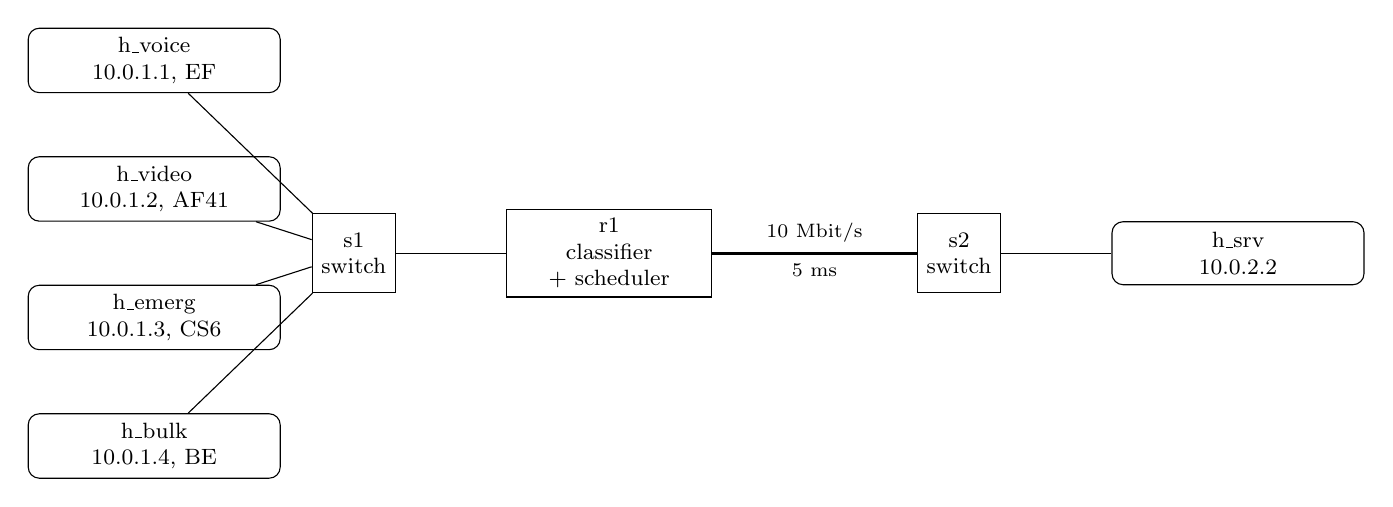
\begin{tikzpicture}[
  node distance=8mm and 14mm,
  host/.style={draw,rounded corners,minimum width=3.2cm,minimum height=0.8cm,align=center,font=\footnotesize},
  box/.style={draw,minimum height=1cm,align=center,font=\footnotesize},
  >=Stealth]
\node[host] (v) {h\_voice\\10.0.1.1, EF};
\node[host,below=of v] (vi) {h\_video\\10.0.1.2, AF41};
\node[host,below=of vi] (e) {h\_emerg\\10.0.1.3, CS6};
\node[host,below=of e] (b) {h\_bulk\\10.0.1.4, BE};
\node[box,right=20mm of $(vi)!0.5!(e)$] (s1) {s1\\switch};
\node[box,right=14mm of s1,minimum width=2.6cm] (r1) {r1\\classifier\\+ scheduler};
\node[box,right=26mm of r1] (s2) {s2\\switch};
\node[host,right=14mm of s2] (srv) {h\_srv\\10.0.2.2};
\foreach \h in {v,vi,e,b} \draw (\h) -- (s1);
\draw (s1) -- (r1);
\draw[very thick] (r1) -- node[above,font=\scriptsize]{10 Mbit/s}node[below,font=\scriptsize]{5 ms}(s2);
\draw (s2) -- (srv);
\end{tikzpicture}
\caption{Proposed topology: four class-specific sources, a classifying/scheduling router and a
10~Mbit/s bottleneck link to the server}\label{fig:topology}
\end{figure}

\textbf{Modules.} The shared Python package \code{qos/} provides the protocol
(\code{protocol.py}), classifier (\code{classifier.py}), schedulers (\code{schedulers.py}), traffic
models, the event-driven bottleneck simulator, metrics and reports. \code{live/} contains the real
UDP sender, software QoS router and receiver; \code{dashboard/} the web interface; \code{tools/}
the pcap verifier; \code{mininet/} the emulation script. Data flows from a sender through the
classifier (which assigns a class) into per-class queues of the scheduler, which releases packets
at the link rate towards the receiver, where one-way delay, jitter and loss are computed.

\subsection{Tools and System Requirements}
\begin{table}[H]\centering\small
\caption{Tools and resources used}\label{tab:tools}
\begin{tabularx}{\textwidth}{|l|l|X|}\hline
\textbf{Tool or resource} & \textbf{Version / specification} & \textbf{Purpose}\\\hline
Python & 3.14.6 (standard library only; project requires 3.8+) & All modules, simulator, tests, dashboard\\\hline
Operating system & macOS (Darwin 25.4.0) & Execution environment for all reported runs\\\hline
Web browser & T3 Code in-app browser, 1280 px wide viewport & Dashboard use and screenshots\\\hline
\code{unittest} & Python standard library & 31 automated tests\\\hline
Wireshark / tshark & Optional; custom Lua dissector \code{docs/qep\_dissector.lua} & Packet-level inspection of QEP\\\hline
Mininet + \code{tc} & Optional, Linux and root required & Emulation script (not executed, see Section~\ref{sec:limitations})\\\hline
\end{tabularx}
\end{table}

\subsection{Addressing and Protocol Selection}
This is a socket and simulation project; the addresses below are those of the Mininet script, in
which the hosts use router \code{r1} (10.0.1.254 on the LAN side, 10.0.2.254 towards the server) as
gateway. The live demo runs all roles on loopback. Table~\ref{tab:addr}
lists them together with the classification keys, and Table~\ref{tab:qep} describes the QEP header.

\begin{table}[H]\centering\small
\caption{Addressing and per-class markings}\label{tab:addr}
\begin{tabularx}{\textwidth}{|l|l|l|X|}\hline
\textbf{Device} & \textbf{IP / DSCP} & \textbf{UDP port} & \textbf{Role (gateway)}\\\hline
h\_voice & 10.0.1.1/24, EF (46) & 5004 & G.711-like voice, 212 B every 20 ms (10.0.1.254)\\\hline
h\_video & 10.0.1.2/24, AF41 (34) & 5006 & 30 fps video, 1252 B packets in bursts (10.0.1.254)\\\hline
h\_emerg & 10.0.1.3/24, CS6 (48) & 5911 & Alarms and sensor events, 172 B (10.0.1.254)\\\hline
h\_bulk & 10.0.1.4/24, BE (0) & 5201, 80, 443, 8080 & Bursty bulk data, 200--1500 B (10.0.1.254)\\\hline
r1 & 10.0.1.254/24, 10.0.2.254/24 & -- & Classifier and scheduler (egress \code{r1-eth2})\\\hline
h\_srv & 10.0.2.2/24 & -- & Receiver (10.0.2.254)\\\hline
\end{tabularx}
\end{table}

\textbf{Protocol choice.} UDP is used because emergency telemetry and voice are delay-sensitive and
retransmission would arrive too late; the QEP header adds what UDP lacks for measurement and
classification. Each datagram is \code{IPv4 (DSCP) | UDP | 24-byte QEP header | payload}.

\begin{table}[H]\centering\small
\caption{QEP header fields (24 bytes)}\label{tab:qep}
\begin{tabularx}{\textwidth}{|l|l|X|}\hline
\textbf{Field} & \textbf{Size} & \textbf{Meaning}\\\hline
Magic & 16 bit & \code{0x5145} (``QE'') identifies QEP\\\hline
Version / Class & 4 + 4 bit & 0 emergency, 1 voice, 2 video, 3 best effort\\\hline
Flags & 8 bit & ALERT (0x01), RETX (0x02), LAST (0x04), PREEMPT\_REQUEST (0x08)\\\hline
Flow ID, DSCP, Reserved & 16 + 8 + 8 bit & Flow identifier; copy of DSCP; reserved\\\hline
Sequence number & 32 bit & Per-flow sequence for loss detection\\\hline
Timestamp & 64 bit & Sender clock in ns since epoch, used for one-way delay\\\hline
Payload length, Checksum & 16 + 16 bit & RFC~1071 \cite{rfc1071} Internet checksum over the header\\\hline
\end{tabularx}
\end{table}

\textbf{Design decisions.} (i) The classifier is staged from the cheapest trustworthy evidence to
the weakest: QEP header, DSCP, UDP port, flow cache, default best effort. DSCP~0 is treated as
``unknown'' because a stripped marking looks identical to best effort. (ii) The flow cache remembers
the class of a flow once any packet was identified, so later packets with stripped markings are
still classified correctly. (iii) Out-of-profile emergency and voice packets are re-marked to best
effort rather than dropped, which bounds the damage of false markings.

%--------------------------------------------------------------------
\section{Implementation and Technical Working}

\subsection{Methodology}
The work proceeded in the following sequence: define the protocol and SLAs; implement the
classifier and the five schedulers behind one interface; build the event-driven bottleneck
simulator with outage, degradation and random-loss models; write the test-case catalogue
(TC1--TC10) and automated tests; add the live UDP pipeline, the dashboard and the pcap tooling;
iterate on the proposed scheduler using failing test cases (Section~\ref{sec:challenges}).

\subsection{Code Implementation}
\textbf{Schedulers} (\code{qos/schedulers.py}) share the interface
\code{enqueue(pkt, now)} $\rightarrow$ dropped packets, and \code{dequeue(now)}.

\begin{table}[H]\centering\small
\caption{Implemented schedulers}\label{tab:sched}
\begin{tabularx}{\textwidth}{|l|X|X|}\hline
\textbf{Name} & \textbf{Description} & \textbf{Weakness it exposes}\\\hline
\code{fifo} & Single tail-drop queue (no QoS baseline) & Everything suffers equally\\\hline
\code{pq} & Strict priority with per-class buffers & Starves low classes; trusts markings\\\hline
\code{wfq} & Self-Clocked Fair Queueing, weights 40/30/20/10 & Emergency only gets its weight under attack\\\hline
\code{drr} & Deficit Round Robin, same weights & Coarser delay (quantum rounds)\\\hline
\code{eps} & Proposed hybrid Emergency Priority Scheduler & Needs call admission control for voice\\\hline
\end{tabularx}
\end{table}

\textbf{EPS} combines: (1) strict top priority for emergency; (2) strict second priority for voice;
(3) video and best effort share the remainder by WFQ in the ratio 6:4 so neither is starved;
(4) policing of tiers 1--2 with a per-flow token bucket and an aggregate class bucket (emergency
20\,\% and voice 35\,\% of the link), where out-of-profile packets are re-marked to best effort; and
(5) a shared buffer with push-out, in which an arriving higher-class packet evicts tail packets of
lower classes when the buffer is full, with per-queue caps for video and best effort to limit
bufferbloat.

\textbf{Metrics} (\code{qos/metrics.py}): one-way delay (average, p50, p95, p99, maximum), jitter
(mean absolute delay variation of consecutive packets per flow), loss, throughput, SLA verdicts,
recovery time (time after a failure ends until emergency delay is again below 100~ms),
classification accuracy and flow-cache hit ratio.

\subsection{Protocols and Technical Working}
In the live demonstration, \code{live/traffic\_sender.py} emits QEP-framed UDP datagrams for each
class. \code{live/qos\_router.py} receives them on the router leg, classifies each packet, enqueues
it in the selected scheduler and a transmit loop paces departures at the configured 1~Mbit/s rate towards
the receiver leg. \code{live/receiver.py} validates the QEP header checksum (corrupted headers are
rejected), reads the sender timestamp and records per-packet delay, from which
\code{live/analyze.py} derives the metrics. Router counters (ingress, egress, dropped per class)
are exposed to the dashboard. Error handling: packets with bad magic, version or checksum are
rejected and counted rather than classified.

\subsection{Execution Procedure}
Prerequisites: Python 3.8 or newer; no packages need to be installed. From the project root:
\begin{lstlisting}
python3 -m unittest -v tests.test_qos           # 31 automated tests
python3 run_simulation.py --scenario all        # all test cases -> results/
python3 live/run_live_demo.py                   # real UDP sockets, 1 Mbit/s router
python3 dashboard/server.py                     # http://127.0.0.1:8080
\end{lstlisting}
The dashboard has a Simulation view (select a test case and press \emph{Run simulation}) and a
Live demo view (choose traffic profile, duration and schedulers and press \emph{Run live demo}).
Figure~\ref{fig:dash-initial} shows the dashboard as launched with the commands above.

\shot{dashboard_initial.png}{Dashboard served at \texttt{http://127.0.0.1:8080} in the in-app browser (before any run)}{fig:dash-initial}

The empty state confirms that the server starts without dependencies and exposes the two views and
the test-case selector listing TC1--TC9.

%--------------------------------------------------------------------
\section{Testing and Results}

\subsection{Test Plan}
The environment is the simulated 10~Mbit/s link (seed 1, 20~s runs; offered load: 20 voice calls,
3 video streams, 10 emergency sources, bulk traffic) and the live 1~Mbit/s software router. The
success criteria are the SLAs of Section~1.4. Normal operation (TC1) and failure or invalid-input
cases (outage, degradation, spoofed markings, noisy markings, link loss) are all included.
Table~\ref{tab:tests} summarises the cases; full per-class tables are in
\code{results/summary\_all.md}.

\begin{table}[H]\centering\scriptsize
\caption{Test plan with observed results (emergency p99 delay / emergency loss, FIFO vs EPS)}\label{tab:tests}
\begin{tabularx}{\textwidth}{|l|p{3.1cm}|X|X|l|}\hline
\textbf{ID} & \textbf{Test and input} & \textbf{Expected result} & \textbf{Observed result} & \textbf{Status}\\\hline
TC1 & Normal load ($\sim$70\,\%) & All schedulers meet every SLA & FIFO emergency p99 42.4 ms; EPS 6.3 ms; all PASS & Pass\\\hline
TC2 & Heavy congestion ($\sim$170\,\%) & FIFO fails SLAs; QoS schedulers pass & FIFO 105.5 ms, 2.91\,\% loss, FAIL; PQ/WFQ/DRR/EPS 6.3--9.8 ms, 0\,\% loss, PASS & Pass\\\hline
TC3 & Disaster surge: 20 sources $\times$ 60 pps for 6 s during congestion & FIFO fails emergency; EPS passes & FIFO 2.54\,\% loss, FAIL; EPS 0\,\% loss, 6.3 ms, PASS & Pass\\\hline
TC4 & 2 s link outage (t = 8--10 s) with emergency event & EPS loses fewest emergency packets & Loss: FIFO 19.9\,\%, PQ/WFQ/DRR 16.4\,\%, EPS 0.0\,\%; recovery FIFO 7163 ms, others $\le$1 ms; whole-run SLA FAIL for all & Partial\\\hline
TC5 & Capacity falls to 35\,\% (t = 6--14 s) & EPS and PQ keep emergency and voice within SLA & EPS voice p99 9.7 ms PASS; WFQ 181.8 ms and DRR 180.5 ms voice FAIL; FIFO all FAIL & Pass\\\hline
TC6 & Bulk flow falsely marked emergency (8 Mbit/s) & EPS holds; others degrade & EPS emergency 0\,\% loss 6.3 ms PASS; PQ video loss 50.2\,\%; PQ/WFQ/DRR emergency FAIL & Pass\\\hline
TC7 & Noisy markings (DSCP stripped 25\,\%, port wrong 10\,\%) & Accuracy rises with each stage & dscp 85.86\,\% $<$ header 88.25\,\% $<$ dscp+port 98.46\,\% $<$ stateless 99.72\,\% $<$ full 100\,\% & Pass\\\hline
TC8 & 90 voice calls (7.6 Mbit/s) & PQ starves; EPS protects video and best effort & PQ best effort 15 kbit/s, video loss 39.2\,\%; EPS video loss 0.07\,\%, but voice loss 20.1\,\% (FAIL) & Partial\\\hline
TC9 & 2\,\% random link loss & Loss in all classes, delay unaffected & About 2\,\% loss in every class; delay unchanged; loss SLA fails by design & Pass\\\hline
TC10 & Load sweep, bulk 1--15 Mbit/s & FIFO delay grows; QoS flat & FIFO 36 $\rightarrow$ 105 ms; PQ/EPS 6.3 ms flat & Pass\\\hline
L1 & Live: congestion (about 190\,\% of 1 Mbit/s) & FIFO fails; QoS pass & Dashboard run: FIFO FAIL/FAIL/FAIL; PQ, WFQ, DRR, EPS PASS/PASS/PASS & Pass\\\hline
L2 & Live: spoofed emergency flood (900 kbit/s) & PQ fails; EPS passes & Dashboard run: PQ, WFQ, DRR emergency and video FAIL; EPS PASS/PASS/PASS & Pass\\\hline
U1 & 31 unit and scenario tests & All pass & \texttt{Ran 31 tests in 5.5s -- OK} & Pass\\\hline
\end{tabularx}
\end{table}

\subsection{Results and Execution Evidence}
All screenshots below were captured from the dashboard running in the in-app browser during this
report's preparation. SLA verdicts are the dashboard's own PASS/FAIL cells, produced by the same
code as the tables above.

\textbf{TC2 -- heavy congestion.} Figure~\ref{fig:tc2} shows FIFO failing emergency, voice and
video while the four QoS schedulers pass. The p99 chart (log scale) shows FIFO's emergency and
voice delay near 100~ms against single-digit milliseconds for the others, and the emergency delay
over time stays flat for every QoS scheduler. Best-effort traffic absorbs the loss (about 53\,\%),
which is the intended trade.

\shot{sim_tc2_congestion.png}{Simulation, TC2 heavy congestion: SLA table, p99 delay, loss, throughput and emergency delay over time}{fig:tc2}

\textbf{TC4 -- outage and recovery.} Figure~\ref{fig:tc4} shows that all schedulers fail the
whole-run SLA because packets that arrive during the 2~s outage are unavoidably delayed, yet the
recovery column differs: FIFO needs 7163~ms before emergency delay is below 100~ms again, whereas
the others recover within 1~ms. The loss chart (not visible in the SLA cells) separates EPS, whose
emergency loss is 0\,\%, from 16--20\,\% for the rest.

\shot{sim_tc4_outage.png}{Simulation, TC4 2 s link outage: recovery time per scheduler}{fig:tc4}

\textbf{TC6 -- spoofed emergency flood.} Figure~\ref{fig:tc6} demonstrates objective O4: when a
bulk flow falsely marked as emergency offers 8~Mbit/s, strict priority, WFQ and DRR fail the
emergency and video SLAs because the flood is served as emergency traffic. EPS passes all three
since per-flow policing re-marks the flood to best effort.

\shot{sim_tc6_spoofed_flood.png}{Simulation, TC6 spoofed emergency flood: only EPS passes all SLAs}{fig:tc6}

\textbf{Live demo -- congestion.} Figure~\ref{fig:live-cong} shows real loopback UDP traffic
through the 1~Mbit/s software router. FIFO drops emergency (20 of 360), voice (31 of 600) and
video (34 of 188) packets, while the four QoS schedulers forward all emergency, voice and video
packets and drop only best-effort traffic. In the stored 8~s run (\code{results/live\_congestion.txt})
FIFO emergency p99 delay was 200.7~ms against 11.9~ms for EPS.

\shot{live_congestion.png}{Live demo, congestion profile: SLA verdicts and software-router packet counters}{fig:live-cong}

\textbf{Live demo -- spoofed flood.} Figure~\ref{fig:live-spoof} repeats the run with a 900~kbit/s
spoofed emergency flood. Strict PQ, WFQ and DRR fail the emergency and video SLAs and only EPS
passes all three. The ``emergency'' counters include the flood itself (852 ingress packets
versus 360 genuine ones in the congestion run), so the large dropped counts there should not be read
as lost genuine alarms; the SLA table, which measures the genuine emergency flows, is the correct
indicator. Stored 8~s numbers: PQ emergency p99 30.3~ms with 0.62\,\% loss (FAIL) versus EPS
13.6~ms with 0\,\% loss (PASS).

\shot{live_spoof.png}{Live demo, spoofed emergency flood: EPS is the only scheduler that passes all SLAs}{fig:live-spoof}

\textbf{Packet-level verification.} \code{tools/pcap\_verify.py} on the TC2 capture analysed 16\,246
QEP packets with 0 header errors and 0 DSCP/class mismatches. With EPS the emergency mean delay was
0.58~ms against 106.21~ms for best effort (``PRIORITY HONOURED''); the FIFO capture showed about
95~ms for every class (``NO PRIORITY EFFECT'').

\subsection{Objective Achievement}
\begin{table}[H]\centering\small
\caption{Objective achievement}\label{tab:achieve}
\begin{tabularx}{\textwidth}{|l|X|l|}\hline
\textbf{ID} & \textbf{Evidence or test ID} & \textbf{Outcome}\\\hline
O1 & TC7 and ablation: accuracy 100\,\% with flow cache, 32.7\,\% of packets served from cache & Achieved\\\hline
O2 & TC2, TC3, L1: emergency p99 6.3 ms and 0\,\% loss for EPS; FIFO fails & Achieved\\\hline
O3 & TC4, TC5: EPS emergency loss 0\,\% in outage, instant recovery; whole-run SLA still fails in TC4 & Partial\\\hline
O4 & TC6, L2: EPS passes; PQ, WFQ, DRR fail. Many-flow-ID attacks only bounded by the aggregate cap & Achieved (single-flow attack)\\\hline
O5 & TC8: EPS video loss 0.07\,\%, best effort 149 kbit/s vs PQ 15 kbit/s; EPS voice loses 20.1\,\% & Partial\\\hline
O6 & TC10 sweep and all comparison tables & Achieved\\\hline
\end{tabularx}
\end{table}

%--------------------------------------------------------------------
\section{Discussion and Conclusion}

\subsection{Discussion and Comparative Analysis}
Table~\ref{tab:compare} compares schedulers on measurable criteria taken from the simulation
results (seed 1). At about 70\,\% load even FIFO meets the SLA, so QoS matters only under
congestion. Under congestion every QoS scheduler protects the low-rate emergency and voice flows;
the differences appear in the harder cases. DRR has the coarsest delay (9.8~ms against 6.3~ms
emergency p99 in TC2) because of round granularity. In TC5, WFQ and DRR let voice exceed its SLA
(about 181~ms) while strict priority and EPS keep it near 10~ms. In TC6, strict priority is the
worst for video (50.2\,\% loss) because it trusts the false marking. In TC8, strict priority
starves best effort. EPS is the only scheduler that passes TC6 and does not starve in TC8, at the
cost of demoting voice beyond its 35\,\% reservation.

\begin{table}[H]\centering\small
\caption{Scheduler comparison (simulation, emergency class unless noted)}\label{tab:compare}
\begin{tabularx}{\textwidth}{|l|X|X|X|X|X|}\hline
\textbf{Criterion} & \textbf{FIFO} & \textbf{PQ} & \textbf{WFQ} & \textbf{DRR} & \textbf{EPS}\\\hline
TC2 p99 delay (ms) & 105.5 & 6.3 & 6.5 & 9.8 & 6.3\\\hline
TC4 loss (\%) / recovery (ms) & 19.9 / 7163 & 16.4 / 1 & 16.4 / 0 & 16.4 / 0 & 0.0 / 0\\\hline
TC5 voice p99 (ms) & 291.5 & 9.6 & 181.8 & 180.5 & 9.7\\\hline
TC6 emergency loss (\%) / video loss (\%) & 1.53 / 24.8 & 0.69 / 50.2 & 2.28 / 28.0 & 4.72 / 27.7 & 0.00 / 0.00\\\hline
TC8 best-effort kbit/s / video loss (\%) & 885 / 56.1 & 15 / 39.2 & 1643 / 8.1 & 1643 / 8.1 & 149 / 0.07\\\hline
\end{tabularx}
\end{table}

\subsection{Advantages and Applications}
The hybrid scheduler gives emergency and voice traffic the delay of strict priority, avoids
starvation of video and best effort, and is robust against a single flow that falsely claims to be
emergency traffic. Applications include disaster-response networks, hospital and public-safety
campus networks, and industrial or utility networks where alarms share links with bulk data. The
protocol, classifier and schedulers are pure Python modules reused unchanged by the simulator, the
live router and the tests.

\subsection{Limitations}\label{sec:limitations}
\begin{itemize}
\item Markings are not authenticated; an attacker using many flow IDs is bounded only by the aggregate cap. An HMAC token or an ingress allow-list would be needed.
\item One bottleneck and UDP-style sources only; no TCP congestion-control feedback and no ECN or AQM (CoDel, RED).
\item The Mininet script (\code{mininet/mn\_qos\_topo.py}) requires Linux and root and was \emph{not executed}; it approximates EPS with HTB (no per-flow policing or push-out in \code{tc}).
\item No call admission control: with 90 voice calls EPS demotes about 20\,\% of voice.
\item Live-demo numbers vary by a few milliseconds with OS scheduling, and the live runs use loopback, not a real network.
\end{itemize}

\subsection{Challenges and Troubleshooting}\label{sec:challenges}
\begin{table}[H]\centering\small
\caption{Issues found during development}\label{tab:issues}
\begin{tabularx}{\textwidth}{|X|X|X|}\hline
\textbf{Issue} & \textbf{Cause / diagnosis} & \textbf{Solution and verification}\\\hline
Genuine alarms demoted under the TC6 flood (p99 307 ms) & First EPS version used only an aggregate emergency policer; the flood consumed the tokens & Added per-flow plus aggregate policing; TC6 now passes\\\hline
Stateless classifier leaked 0.3--0.5\,\% of packets to best effort (TC7 emergency loss 0.12\,\%) & Stripped or wrong markings could not be recovered per packet & Added flow cache; accuracy 100\,\%, emergency loss 0\,\%\\\hline
Video filled the whole shared buffer under degradation (p99 885 ms) & No per-queue cap in the shared buffer & Per-queue caps for video and best effort\\\hline
Live-demo profiles too generous for a 1 Mbit/s link & Policer profiles were sized for 10 Mbit/s & Profiles scaled to the link; live results ordering stable\\\hline
\end{tabularx}
\end{table}

\subsection{Future Scope}
Authenticated emergency markings (HMAC token in the QEP reserved field), call admission control for
voice, multi-hop topologies, AQM/ECN, forward error correction or retransmission using the QEP RETX
flag for lossy links, and executing the Mininet emulation on a Linux host.

\subsection{Conclusion}
The project delivered a protocol, classifier, five schedulers, a simulator with nine test cases and
a load sweep, a live UDP pipeline, a dashboard and packet-level tooling. Objectives O1, O2, O4 and
O6 were achieved, and O3 and O5 partially: in the outage test every scheduler fails the whole-run
SLA, and EPS protects video and best effort in the starvation test but loses voice beyond its
reservation. The proposed EPS was the only scheduler to pass the spoofed-flood test in both the
simulation and the live run. The unit-test suite (31 tests) passed.

%====================================================================
\newpage
\section*{References}
\addcontentsline{toc}{section}{References}
\begin{thebibliography}{9}
\bibitem{rfc2474} K. Nichols, S. Blake, F. Baker and D. Black, ``Definition of the Differentiated Services Field (DS Field) in the IPv4 and IPv6 Headers,'' RFC 2474, IETF, Dec. 1998. [Online]. Available: https://www.rfc-editor.org/rfc/rfc2474
\bibitem{rfc2475} S. Blake, D. Black, M. Carlson, E. Davies, Z. Wang and W. Weiss, ``An Architecture for Differentiated Services,'' RFC 2475, IETF, Dec. 1998. [Online]. Available: https://www.rfc-editor.org/rfc/rfc2475
\bibitem{rfc3246} B. Davie \emph{et al.}, ``An Expedited Forwarding PHB (Per-Hop Behavior),'' RFC 3246, IETF, Mar. 2002. [Online]. Available: https://www.rfc-editor.org/rfc/rfc3246
\bibitem{demers1989} A. Demers, S. Keshav and S. Shenker, ``Analysis and simulation of a fair queueing algorithm,'' in \emph{Proc. ACM SIGCOMM}, 1989, pp. 1--12.
\bibitem{shreedhar1996} M. Shreedhar and G. Varghese, ``Efficient fair queueing using deficit round-robin,'' \emph{IEEE/ACM Trans. Networking}, vol. 4, no. 3, pp. 375--385, 1996.
\bibitem{rfc1071} R. Braden, D. Borman and C. Partridge, ``Computing the Internet Checksum,'' RFC 1071, IETF, Sep. 1988. [Online]. Available: https://www.rfc-editor.org/rfc/rfc1071
\end{thebibliography}

\section*{AI Usage Declaration}
\addcontentsline{toc}{section}{AI Usage Declaration}
\textbf{AI tools used:} Claude Code, accessed through T3 Code.

\textbf{Purpose:} Claude Code was used for AI-assisted testing (launching the project's dashboard,
running the simulation and live-demo scenarios and the unit tests, and capturing the screenshots in
the figures) and for drafting this report from the project's source files, README and result files.
It also suggested the cited references.

\textbf{Verification by the group:} The group also carried out its own tests of the project in
addition to the AI-assisted testing. The numbers in the report come from the stored result files
(\code{results/summary\_all.md}, \code{results/live\_*.txt}, \code{results/pcap\_verify\_*.txt}) and
from the dashboard runs and the 31-test unit run performed during preparation. The Mininet script
was not executed by either the group or the AI tool, and no results are claimed for it.

\medskip
\textbf{Declaration:} We take responsibility for the accuracy of this report and understand the
submitted implementation and results. Sources and assistance used have been acknowledged.

\begin{center}
\begin{tabular}{|l|l|l|}\hline
\textbf{Student Name} & \textbf{PRN} & \textbf{Signature}\\\hline
Kaustubh Dube & 1262254051 & \\\hline
Abhiram Tawalare & 1262241934 & \\\hline
Shalaka Bhor & 1262242503 & \\\hline
Charitra Jain & 1262243266 & \\\hline
\end{tabular}
\end{center}

%====================================================================
\newpage
\section*{Appendices}
\addcontentsline{toc}{section}{Appendices}

\subsection*{Appendix A \quad Code and Configuration}
Complete source is in the project repository. Key files:
\code{qos/protocol.py} (QEP framing and checksum), \code{qos/classifier.py} (staged classifier),
\code{qos/schedulers.py} (FIFO, PQ, WFQ, DRR, EPS), \code{qos/simulator.py}, \code{qos/scenarios.py}
(test-case catalogue), \code{live/qos\_router.py}, \code{dashboard/server.py},
\code{tools/pcap\_verify.py}, \code{docs/qep\_dissector.lua} and \code{tests/test\_qos.py}.
The test-case configuration shared by the scenarios is:
\begin{lstlisting}
BASE = dict(
    duration=20.0, link_bps=10e6, prop_delay=0.005, buffer_bytes=125000,
    loss_prob=0.0, profile=[],
    voice_calls=20, video_streams=3, video_kbps=3000,
    emerg_sources=10, emerg_hb_pps=10, emerg_events=[(5.0, 3.0, 40)],
    be_kbps=2000, spoof_kbps=0, noise={}, classifier="full", sched_opts={},
)
\end{lstlisting}

\subsection*{Appendix B \quad Additional Evidence}
Stored 8~s live-demo results (1~Mbit/s router, about 190\,\% offered load), from
\code{results/live\_congestion.txt}:
\begin{table}[H]\centering\small
\caption{Live demo, congestion profile (stored run)}\label{tab:live}
\begin{tabular}{|l|r|r|r|l|}\hline
\textbf{Scheduler} & \textbf{EM p99 (ms)} & \textbf{EM loss (\%)} & \textbf{Voice p99 (ms)} & \textbf{SLA EM/VO/VI}\\\hline
FIFO & 200.7 & 3.33 & 202.2 & F/F/F\\\hline
Strict PQ & 12.0 & 0.00 & 14.7 & P/P/P\\\hline
WFQ & 13.8 & 0.00 & 13.7 & P/P/P\\\hline
DRR & 38.3 & 0.00 & 36.4 & P/P/P\\\hline
EPS & 11.9 & 0.00 & 15.1 & P/P/P\\\hline
\end{tabular}
\end{table}
Classifier ablation (TC7 noise), from the same result set:
\begin{table}[H]\centering\small
\caption{Classifier ablation under noisy markings}\label{tab:ablation}
\begin{tabular}{|l|r|r|r|}\hline
\textbf{Mode} & \textbf{Accuracy (\%)} & \textbf{EM loss (\%)} & \textbf{EM p99 (ms)}\\\hline
DSCP only & 85.86 & 1.23 & 117\\\hline
DSCP + port & 98.46 & 0.23 & 117\\\hline
Header only & 88.25 & 1.41 & 118\\\hline
Header + DSCP + port (stateless) & 99.72 & 0.00 & 6.3\\\hline
+ flow cache (full) & 100.00 & 0.00 & 6.3\\\hline
\end{tabular}
\end{table}

\subsection*{Appendix C \quad Individual Contributions}
\begin{table}[H]\centering\small
\caption{Individual contributions (implementation split)}\label{tab:contrib}
\begin{tabularx}{\textwidth}{|l|X|X|}\hline
\textbf{Student name and PRN} & \textbf{Work completed} & \textbf{Evidence or deliverable}\\\hline
Kaustubh Dube (1262254051) & Web dashboard (Simulation and Live demo views); synthetic traffic generators; test-case catalogue; running and maintaining the automated test suite & \code{dashboard/}, \code{qos/traffic.py}, \code{qos/scenarios.py}, \code{tests/test\_qos.py} (31 tests); Figures~\ref{fig:dash-initial}--\ref{fig:live-spoof}\\\hline
Abhiram Tawalare (1262241934) & QEP protocol (24-byte header, RFC 1071 checksum); staged packet classifier with flow cache; delay, jitter, loss and SLA metrics; pcap writer/reader and packet-level verifier & \code{qos/protocol.py}, \code{qos/classifier.py}, \code{qos/metrics.py}, \code{qos/pcapio.py}, \code{tools/pcap\_verify.py}; Tables~\ref{tab:qep} and~\ref{tab:ablation}\\\hline
Shalaka Bhor (1262242503) & Live UDP pipeline: software QoS router, traffic sender, receiver and one-command demo; baseline schedulers FIFO, strict priority, WFQ and DRR & \code{live/}, \code{FIFO}, \code{StrictPriority}, \code{WFQ} and \code{DRR} in \code{qos/schedulers.py}; Figures~\ref{fig:live-cong} and~\ref{fig:live-spoof}\\\hline
Charitra Jain (1262243266) & Proposed Emergency Priority Scheduler (per-flow and aggregate token-bucket policing, re-marking, push-out shared buffer); discrete-event simulator with outage, degradation and loss models & \code{EPS} and \code{TokenBucket} in \code{qos/schedulers.py}, \code{qos/simulator.py}; Tables~\ref{tab:tests} and~\ref{tab:compare}\\\hline
\end{tabularx}
\end{table}

\end{document}
